\chapter{HASIL DAN PEMBAHASAN}
\section{Hasil Perancangan Sistem}
Sistem deteksi ini dirancang secara otomatis
menggunakan kamera sebagai sensor utama dan lengan robot sebagai
aktuator. Proses diawali dengan model YOLO yang mengidentifikasi
keberadaan kontainer dari \textit{input} kamera. Jika kontainer terdeteksi,
citra akan dianalisis oleh model \textit{autoencoder} untuk mengklasifikasikan
adanya kecacatan. Berdasarkan hasil klasifikasi tersebut, lengan
robot yang digerakkan \textit{servo} akan menyortir kontainer ke dalam
kategori cacat atau non-cacat. Secara terpisah, sensor PIR berfungsi
menghitung jumlah total
kontainer pada setiap kategori, di mana data tersebut kemudian
dikirim \textit{web-server} untuk visualisasi pada sisi
klien melalui \textit{dashboard} berbasis \textit{website}. Desain
sistem yang dirancang diilustrasikan pada Gambar \ref{fig:rancang-sistem}.

\begin{figure}[H]
  \centering
  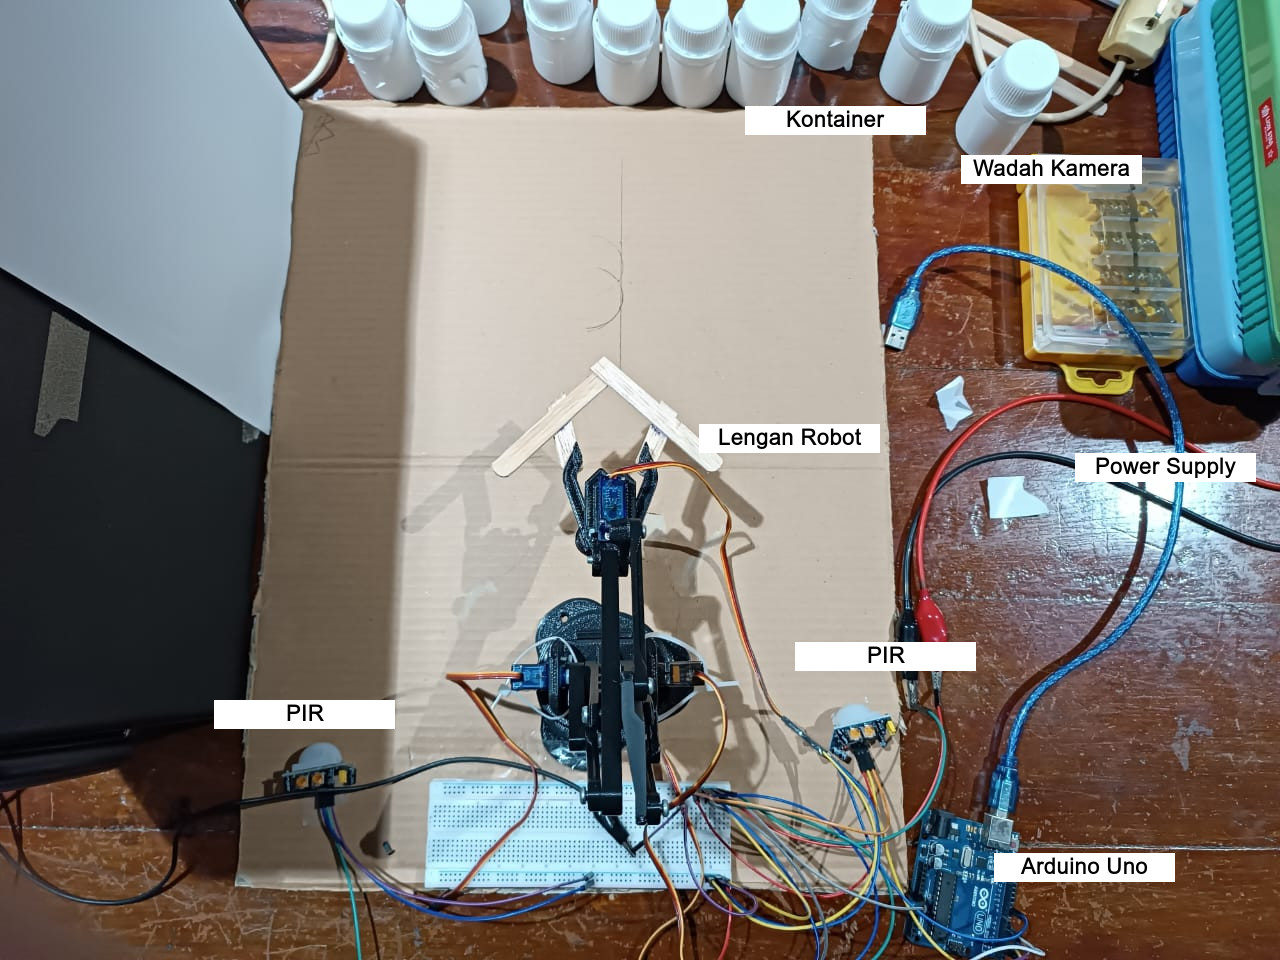
\includegraphics[width=\textwidth]{gambar/rancang_sistem.jpg}
  \caption{Hasil perancangan sistem}
  \label{fig:rancang-sistem}
\end{figure}
\vspace{-1em}

\vspace{1em}

\section{Hasil Perancangan Model YOLO}
\subsection{\textit{Dataset} dan \textit{Preprocessing}}
Tahap awal dalam penelitian ini adalah pengumpulan data primer berupa
citra kontainer menggunakan kamera. Proses akuisisi data dilakukan
untuk membangun sebuah \textit{dataset} kustom yang merepresentasikan objek
target secara akurat. Total gambar mentah yang berhasil dikumpulkan
adalah 463 citra. Pengambilan gambar dilakukan dengan melakukan
variasi terhadap lokasi kontainer untuk memastikan model yang akan
dilatih nantinya mampu mengenali objek dengan baik. \textit{Dataset} kemudian
dibagi menjadi 395 gambar untuk data latih dan 68 data validasi.
Distribusi pembagian \textit{dataset} disajikan pada Tabel
\ref{tab:pembagian-dataset}.

\begin{table}[H]
  \caption{Distribusi pembagian \textit{dataset}}
  \label{tab:pembagian-dataset}
  \vspace{-1em}
  \centering
  \begin{tabular}{ccc}
    \toprule
    \textbf{Kategori} & \textbf{Jumlah Gambar} & \textbf{Persentase} \\
    \midrule
    Data Latih & 395 & 85,3\% \\
    Data Validasi & 68 & 14,7\% \\
    Total Data & 463 & 100\% \\
    \bottomrule
  \end{tabular}
\end{table}

Setelah tahap akuisisi data, proses selanjutnya adalah anotasi
gambar. Anotasi merupakan proses fundamental untuk menghasilkan
\textit{dataset} berlabel yang
akan digunakan sebagai data pelatihan \citep{19}. Dalam
konteks penelitian ini, anotasi dilakukan dengan memberikan
\textit{bounding box} serta label kelas pada setiap objek di dalam
gambar. Metode ini sangat penting karena arsitektur YOLO dirancang
untuk memprediksi \textit{bounding box} dan probabilitas kelas secara
bersamaan sehingga memerlukan data latih dengan format spesifik
tersebut \citep{20}. Sebanyak 463 gambar kontainer telah
dianotasi secara manual. Contoh hasil anotasi dapat dilihat pada Gambar
\ref{fig:yolo-anotasi}.

\begin{figure}[H]
  \centering
  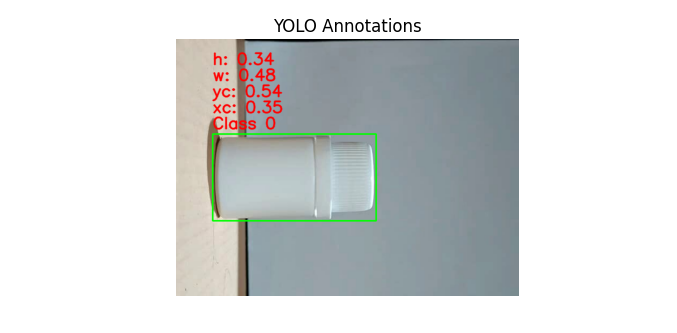
\includegraphics[width=0.7\textwidth]{gambar/anotasi.png}
  \caption{Salah satu data \textit{train} dengan labelnya}
  \label{fig:yolo-anotasi}
\end{figure}
\vspace{-1em}

\vspace{1em}

\subsection{Hasil Pelatihan Model}
Pada penelitian ini, \textit{mean Average Precision} (mAP) digunakan
sebagai metrik utama untuk mengukur performa model YOLO. Akurasi
deteksi ini sangat penting agar lengan robot dapat melakukan inspeksi
kecacatan secara tepat. Metrik ini dihitung berdasarkan
\textit{Average Precision} (AP), yang merupakan kombinasi dari
\textit{precision} dan \textit{recall} untuk setiap kelas secara
individual. Nilai mAP
sendiri adalah rata-rata AP untuk semua kelas, sehingga mampu
memberikan gambaran performa model yang komprehensif \citep{21}. \par

Untuk menentukan apakah sebuah prediksi dianggap benar (\textit{True
Positive}) atau salah (\textit{False Positive}), digunakan metrik
\textit{Intersection over Union} (IoU). IoU merupakan rasio antara area
tumpang tindih (\textit{overlap}) dari \textit{bounding box} hasil prediksi
($BB_{predict}$) dengan
\textit{bounding box ground truth} ($BB_{ground}$), dengan nilai berkisar antara
0 hingga 1 \citep{22}.
Semakin mendekati 1, berarti prediksi semakin akurat dan sesuai
dengan objek sebenarnya. IoU dihitung menggunakan persamaan:
\begin{equation}
  IoU = \frac{|BB_{predict} \cap
  BB_{ground}|}{|BB_{predict} \cup BB_{ground}|}
\end{equation}
\indent
\textit{Precision} mengukur proporsi prediksi positif yang benar (\textit{True
Positive}) terhadap seluruh prediksi positif (TP + \textit{False
Positive}), sehingga menunjukkan kemampuan model dalam meminimalkan kesalahan
deteksi. Sementara itu, \textit{recall} atau \textit{true positive
rate} mengukur seberapa banyak \textit{instance} positif sebenarnya yang
berhasil dideteksi \citep{23}. \textit{Precision} dan
\textit{recall} dapat dihitung menggunakan persamaan:
\begin{equation}
  Precision = \frac{TP}{TP + FP}, \quad
  Recall = \frac{TP}{TP + FN}
\end{equation}
Model YOLO yang digunakan dalam penelitian ini hanya
memprediksi satu kelas yaitu kontainer kimia, maka nilai mAP setara
dengan nilai AP. Nilai AP dihitung sebagai rata-rata
\textit{precision} di seluruh
rentang nilai \textit{recall} (0 hingga 1) \citep{24}, sebagaimana
dirumuskan dalam
Persamaan 3, di mana P adalah \textit{precision} dan r adalah \textit{recall}.
\begin{equation}
  AP = \int_{0}^{1} P(r) \,dr
\end{equation}
\indent
Proses pelatihan model YOLO dilakukan menggunakan \textit{platform}
\textit{Google
Colaboratory}. Model dilatih secara iteratif selama 50 \textit{epoch} dengan
\textit{batch size} 16 dan \textit{optimizer} Adam, agar model dapat mempelajari
fitur-fitur dari data latih secara optimal. Hasil pelatihan model
YOLO setiap 10 \textit{epoch} dapat dilihat pada Tabel \ref{tab:yolo-train}.
\begin{table}[H]
  \caption{Proses \textit{training} model YOLO}
  \label{tab:yolo-train}
  \vspace{-1em}
  \centering
  \small
  \begin{tabular}{c p{1.5cm} p{1.5cm} p{1.5cm} p{1.5cm} p{1.5cm} p{1.5cm}}
    \toprule
    \textbf{Epoch} & \textbf{Train/Box Loss} & \textbf{Train/Class Loss}
    & \textbf{Train/DFL Loss} & \textbf{Val/Box Loss}
    & \textbf{Val/Class Loss} & \textbf{Val/DFL Loss} \\
    \midrule
    0  & 0,5946 & 1,9374 & 0,9706 & 0,4709 & 2,5029 & 0,8990 \\
    10 & 0,4333 & 0,4356 & 0,8713 & 0,3052 & 0,3758 & 0,8262 \\
    20 & 0,3286 & 0,2935 & 0,8510 & 0,3342 & 0,2105 & 0,8448 \\
    30 & 0,2821 & 0,2328 & 0,8390 & 0,2418 & 0,1566 & 0,8244 \\
    40 & 0,2267 & 0,1776 & 0,8010 & 0,2209 & 0,1386 & 0,8201 \\
    50 & 0,2016 & 0,1546 & 0,7993 & 0,2003 & 0,1163 & 0,8156 \\
    \bottomrule
  \end{tabular}
  \normalsize
\end{table}
Pada proses \textit{training}, nilai \textit{loss} pada data
\textit{train} dan validasi secara umum menunjukkan tren penurunan
seiring bertambahnya \textit{epoch}. Penurunan ini menunjukkan bahwa
model semakin mampu menyesuaikan parameter internalnya dengan data
yang diberikan. Dengan demikian, model menjadi lebih baik dalam
mempelajari pola yang relevan untuk mendeteksi kontaier.

Pada \textit{Train/Box Loss}, terjadi penurunan signifikan dari
0,5946 pada \textit{epoch} ke-0 menjadi 0,2016 pada \textit{epoch}
ke-50, yang mengindikasikan peningkatan kemampuan model dalam
memprediksi posisi \textit{bounding box} secara lebih akurat. Hal
serupa juga terlihat pada \textit{Train/Class Loss}, yang turun
drastis dari 1,9374 menjadi 0,1546, menandakan model semakin tepat
dalam melakukan klasifikasi objek. Sementara itu, \textit{Train/DFL
Loss (Distribution Focal Loss)} menurun dari 0,9706 menjadi 0,7993,
yang berarti model semakin baik dalam memperbaiki distribusi prediksi
\textit{bounding box}. Pada data validasi, \textit{Val/Box Loss}
menurun dari 0,4709 ke 0,2003, \textit{Val/Class Loss} dari 2,5029
ke 0,1163, serta \textit{Val/DFL Loss} dari 0,89890 ke 0,8156.
Penurunan yang konsisten pada semua komponen \textit{loss} validasi
menunjukkan bahwa model tidak hanya mampu belajar dengan baik pada
data \textit{train}, tetapi juga memiliki kemampuan generalisasi yang
baik pada data validasi.

Namun, penilaian kinerja model tidak dapat semata-mata bergantung
pada nilai \textit{loss}. Diperlukan metrik tambahan seperti mAP
untuk mengevaluasi akurasi deteksi serta kualitas prediksi
\textit{bounding box} secara keseluruhan. Pada penelitian ini
digunakan mAP@50 (IoU ambang batas 50\%) untuk mengukur
keberhasilan deteksi secara lebih longgar, serta mAP@95 (rata-rata
mAP dari IoU ambang batas 50\% hingga 95\% dengan interval 5\%)
untuk menilai ketepatan prediksi \textit{bounding box} secara lebih
ketat dan detail. Hasil pengukuran mAP pada tiap \textit{epoch} dapat
dilihat pada Gambar \ref{fig:map}.

\begin{figure}[H]
  \centering
  % First image
  \begin{minipage}[]{\textwidth}
    \centering
    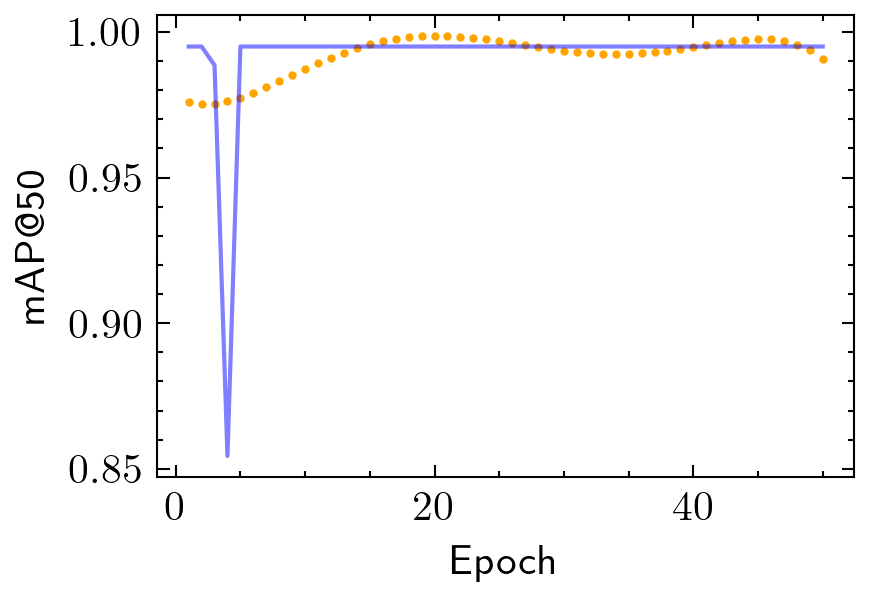
\includegraphics[width=0.8\textwidth]{gambar/map50.png}
    (a)
  \end{minipage}
  \vspace{1em}

  % Second image
  \begin{minipage}{\textwidth}
    \centering
    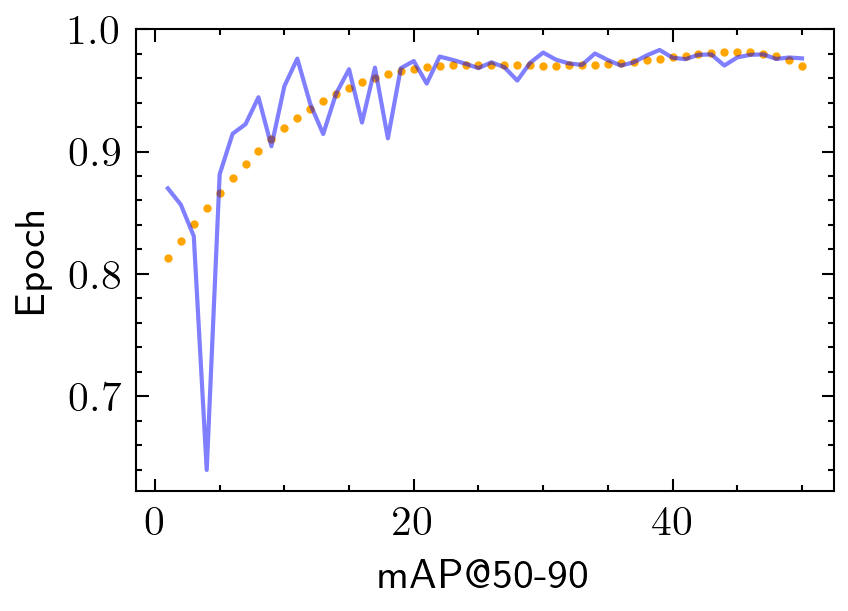
\includegraphics[width=0.8\textwidth]{gambar/map5090.png}
    (b)
  \end{minipage}
  \caption{Grafik tren mAP: (a) mAP@50, (b) mAP@50-90}
  \label{fig:map}
  \vspace{-1em}
\end{figure}

Grafik tersebut menyajikan evaluasi performa model deteksi objek
menggunakan metrik mAP seiring berjalannya
50 \textit{epoch} pelatihan. Grafik di sebelah kiri, mAP@50, yang menggunakan
ambang batas IoU longgar (50\%), menunjukkan bahwa model dengan
sangat cepat mencapai performa puncak. Terlihat bahwa nilainya
melonjak mendekati 1 hanya dalam 10-15 \textit{epoch} pertama lalu
cenderung datar, menandakan model mampu mempelajari cara mendeteksi
keberadaan objek secara umum dengan sangat cepat. Sebaliknya, grafik
di sebelah kanan, mAP@50-95, yang mengukur performa pada rentang
ambang batas IoU yang lebih ketat (50\% hingga 95\%), menunjukkan
kurva pembelajaran yang lebih bertahap dan konsisten. Peningkatan
yang lebih landai ini mengindikasikan bahwa model menggunakan
mayoritas waktu pelatihannya untuk terus-menerus menyempurnakan
presisi dan akurasi lokalisasi \textit{bounding box}-nya. Secara keseluruhan,
pencapaian nilai mAP yang sangat tinggi pada kedua metrik di akhir
pelatihan menandakan model final yang dihasilkan tidak hanya mampu
mendeteksi objek, tetapi juga sangat akurat dalam menentukan
batas-batasnya. Hasil deteksi kontainer kimia pada data validasi
dapat dilihat pada Gambar \ref{fig:yolo-validasi}.

\begin{figure}[H]
  \centering
  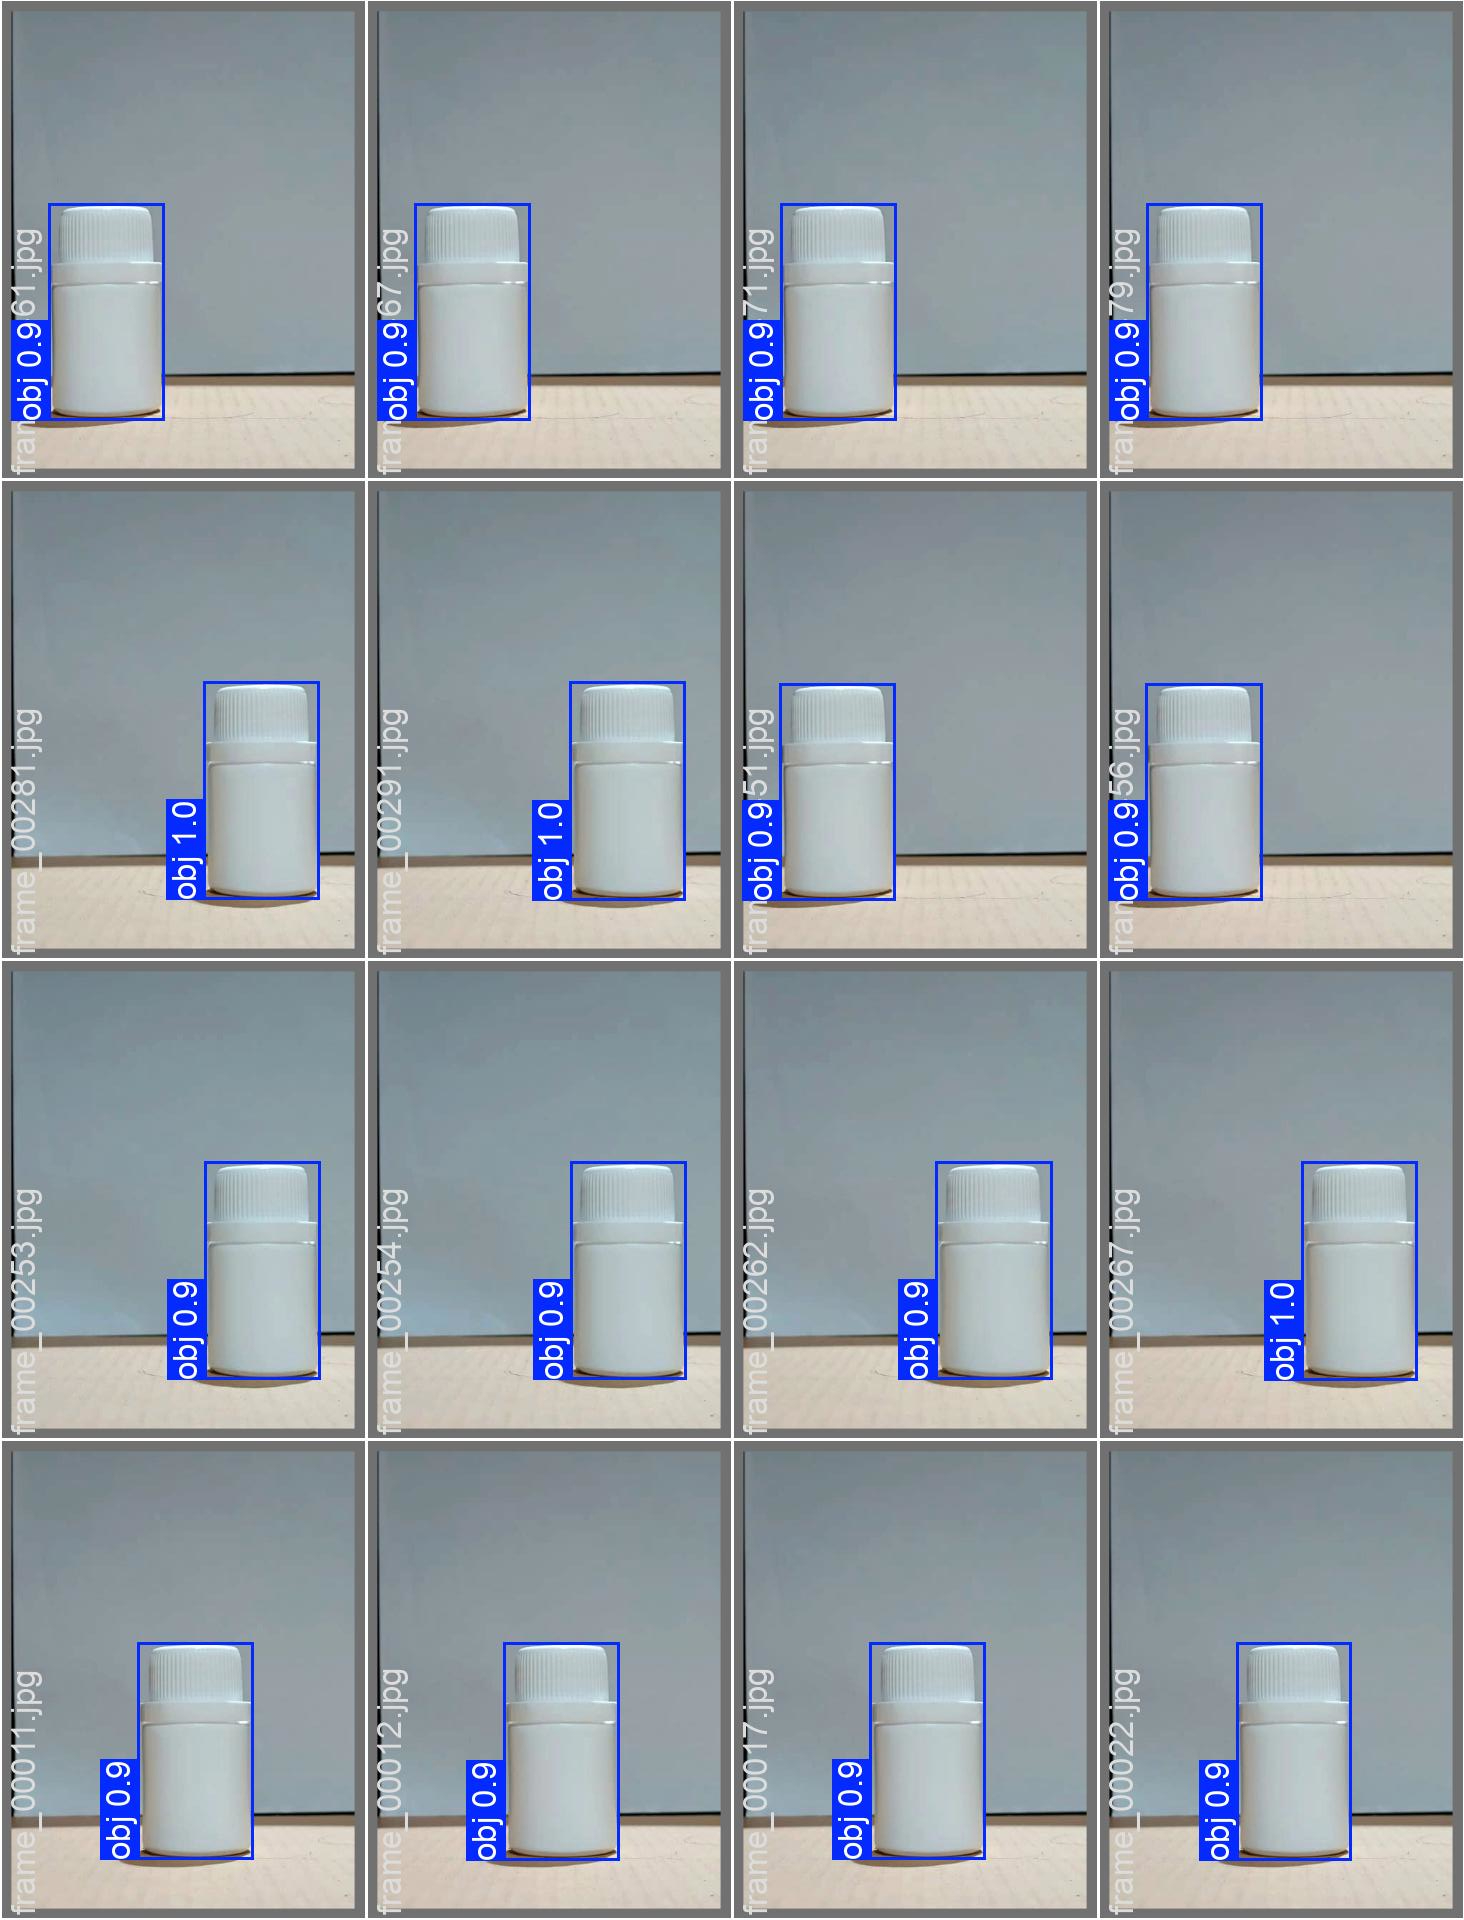
\includegraphics[width=0.93\textwidth]{gambar/yolo_validasi.jpg}
  \caption{Hasil prediksi YOLO pada data validasi}
  \label{fig:yolo-validasi}
\end{figure}
\vspace{-1em}

\vspace{1em}

\section{Hasil Perancangan Model Deteksi Kecacatan}
\subsection{Arsitektur Variational Autoencoder}
\textit{Variational autoencoder} (VAE) merupakan pengembangan dari
\textit{autoencoder}, yaitu sebuah arsitektur \textit{neural network}
yang berfungsi untuk mengekstrak fitur laten dari data. Perbedaan
fundamental VAE dibandingkan pendahulunya terletak pada pendekatan
Bayesian, di mana vektor laten ($z$) dipaksa mengikuti distribusi
probabilitas terstruktur, umumnya distribusi Gaussian. Secara
operasional, \textit{encoder} VAE ($q_{\phi}(z \mid x)$) tidak hanya
mengompres data \textit{input} ($x$), melainkan juga memetakannya
ke dalam parameter statistik: sebuah vektor \textit{mean} dan
vektor varians. Selanjutnya, sebuah sampel kode laten ($z$) diambil
dari distribusi yang diwakili oleh kedua parameter ini, lalu diumpankan
ke \textit{decoder} ($p_{\theta}(x \mid z)$) untuk merekonstruksi
data \textit{input}
asli \citep{25}. Arsitektur \textit{variational autoencoder} yang digunakan pada
penelitian ini dapat dilihat pada Gambar \ref{fig:arsitektur-autoencoder}.

\begin{figure}[H]
  \centering
  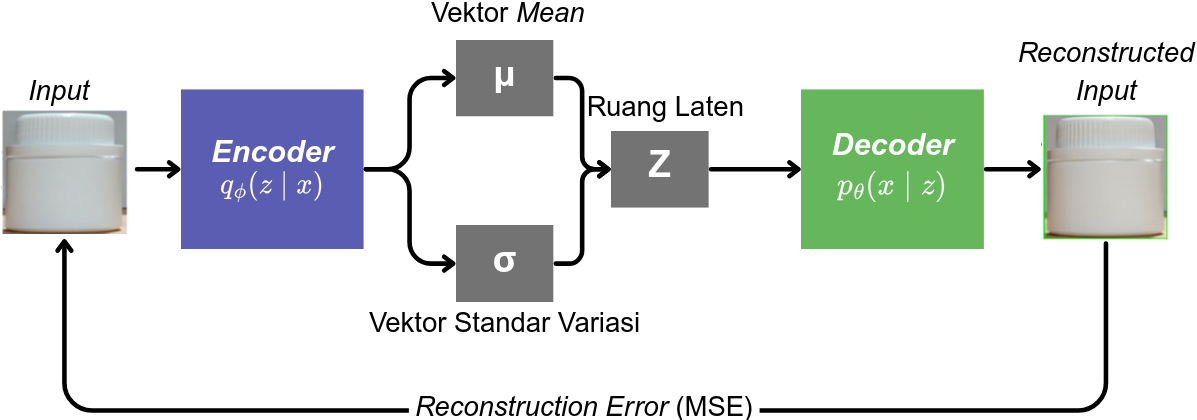
\includegraphics[width=\textwidth]{gambar/arsitektur_autoencoder.png}
  \caption{Arsitektur \textit{variational autoencoder}}
  \label{fig:arsitektur-autoencoder}
\end{figure}
\vspace{-1em}

Arsitektur VAE yang diimplementasikan pada penelitian ini dirancang
untuk memproses citra berukuran 128 $\times$ 128 dengan tiga kanal
warna (RGB). Bagian \textit{encoder} menggunakan lima lapis
\textit{convolutional} berurutan, masing-masing diikuti fungsi
aktivasi ReLU, untuk mengekstrak dan menurunkan
resolusi fitur spasial, hingga menghasilkan representasi akhir
berukuran (512, 4, 4). Representasi ini kemudian diproyeksikan
menjadi dua vektor, yaitu vektor
\textit{mean} dan vektor \textit{log-varians}, yang mendefinisikan
distribusi Gaussian
multivariat sebagai ruang laten. Setelah \textit{sampling} vektor laten $z$,
\textit{decoder} memproyeksikan kembali $z$ ke dimensi spasial melalui lapisan
linear dan serangkaian lapisan \textit{transpose convolutional}
(dekonvolusi) yang secara bertahap memperbesar resolusi hingga
kembali ke ukuran asli citra \textit{input}. Fungsi aktivasi sigmoid pada
lapisan output memastikan nilai piksel berada pada rentang $\text{[0, 1]}$,
sehingga hasil rekonstruksi dapat diinterpretasikan sebagai citra valid.

\vspace{1em}

\subsection{\textit{Dataset} dan \textit{Preprocessing}}
Tahap ini adalah pengumpulan data primer berupa
citra kontainer menggunakan kamera. Proses akuisisi data ini
dilakukan untuk membangun \textit{dataset} kustom yang secara spesifik
merepresentasikan objek target. Total gambar mentah yang berhasil
dikumpulkan berjumlah 3005 citra, yang seluruhnya digunakan sebagai
\textit{dataset} latih. Sebelum digunakan untuk pelatihan
\textit{autoencoder}, seluruh
citra diproses menggunakan model YOLO untuk mendeteksi serta
melakukan \textit{cropping} area kontainer
secara otomatis. Dengan demikian, hanya bagian kontainer yang relevan
yang masuk ke alur pemrosesan, sehingga model \textit{autoencoder} dapat
lebih fokus dalam mempelajari fitur visual kontainer secara mendalam.
Contoh salah satu data dapat dilihat pada Gambar \ref{fig:ae-data}.

\begin{figure}[H]
  \centering
  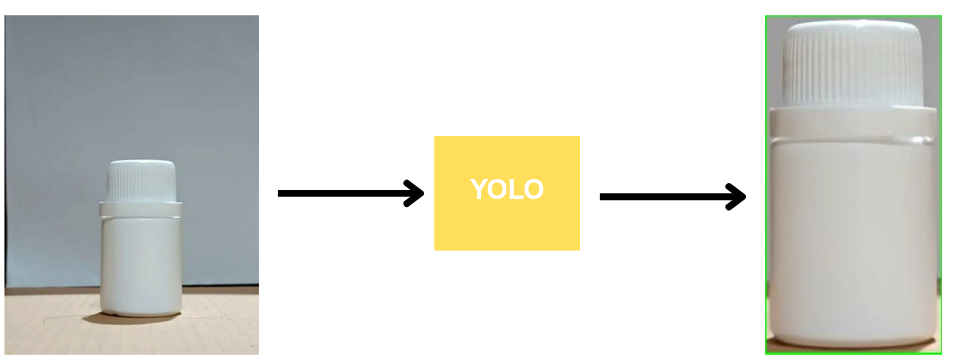
\includegraphics[width=\textwidth]{gambar/ae_data.png}
  \caption{Salah satu data latih model \textit{autoencoder}}
  \label{fig:ae-data}
\end{figure}
\vspace{-1em}

Karena \textit{autoencoder} termasuk dalam kategori \textit{unsupervised
learning}, data yang digunakan pada penelitian ini tidak memerlukan
label atau anotasi manual. Seluruh data pada \textit{dataset} terdiri
dari citra kontainer dalam kondisi bebas cacat visual, sehingga model
\textit{autoencoder} dapat belajar merepresentasikan
distribusi citra kontainer normal secara optimal. Dengan demikian,
\textit{autoencoder} akan berfokus pada rekonstruksi citra
\textit{input} semirip
mungkin, dan nantinya dapat digunakan untuk mendeteksi anomali atau
kerusakan berdasarkan perbedaan signifikan antara citra asli dan
hasil rekonstruksi.

\vspace{1em}

\subsection{Hasil Pelatihan Model}

Fungsi \textit{loss} VAE didasarkan pada \textit{Evidence Lower
Bound} (ELBO). Tujuannya
adalah memaksimalkan \textit{bound} ini agar dapat mengatasi masalah
distribusi posterior yang tidak dapat dihitung secara langsung pada
model probabilistik. Fungsi \textit{loss} terdiri dari dua komponen utama.
Komponen pertama adalah \textit{reconstruction loss}, yang merupakan
ekspektasi dari error rekonstruksi negatif. Komponen ini mengukur
seberapa baik \textit{decoder} probabilistik, $p_\theta(x|z)$, dapat
merekonstruksi data \textit{input} $x$ dari representasi laten $z$. Komponen
kedua adalah \textit{regularization term}, yang dihitung sebagai
Kullback-Leibler (KL) \textit{divergence} antara distribusi posterior
aproksimasi $q_\phi(z|x)$ dan distribusi prior $p_\theta(z)$.
Komponen ini berfungsi sebagai penalti, supaya distribusi yang
dihasilkan \textit{encoder} tetap mendekati distribusi prior sederhana
seperti distribusi Gaussian \citep{26}. Fungsi \textit{loss}
VAE dapat ditulis sebagai:
\begin{equation}
  \mathcal{L}(\theta, \phi; x) = \mathbb{E}{q\phi(z|x)}[\log
  p_\theta(x|z)] - D_{KL}(q_\phi(z|x) \parallel p_\theta(z))
\end{equation}
\indent
Proses pelatihan model CVAE dilakukan
menggunakan komputer dengan GPU NVIDIA GeForce RTX 3050 8GB VRAM
untuk memanfaatkan kemampuan komputasi paralel CUDA. Model dilatih
secara iteratif selama 100 \textit{epoch} dengan
\textit{batch size} 64
dan \textit{optimizer} Adam, agar model dapat mempelajari fitur-fitur
dari data latih secara optimal. Hasil pelatihan model YOLO setiap 10
\textit{epoch} dapat dilihat pada Tabel \ref{tab:training-autoencoder}.

\begin{table}[H]
  \caption{Proses \textit{training} model model \textit{convolutional
  variational autoencoder} (CVAE)}
  \label{tab:training-autoencoder}
  \vspace{-1em}
  \centering
  \begin{tabular}{cc}
    \toprule
    \textbf{Epoch} & \textbf{Loss} \\
    \midrule
    1 & 837,7615 \\
    10 & 30,5440 \\
    20 & 22,6941 \\
    30 & 18,5220 \\
    40 & 15,0172 \\
    50 & 11,9098 \\
    60 & 9,8593 \\
    70 & 8,7772 \\
    80 & 7,3923 \\
    90 & 7,1070 \\
    100 & 6,8338 \\
    \bottomrule
  \end{tabular}
\end{table}
Pada proses \textit{training}, nilai \textit{loss} rekonstruksi
secara umum menunjukkan tren penurunan seiring bertambahnya
\textit{epoch}. Penurunan ini mengindikasikan bahwa model \textit{autoencoder}
semakin mampu mempelajari representasi fitur penting dari data normal
yang diberikan. Dengan demikian, model menjadi lebih baik dalam
merekonstruksi kontainer kimia tanpa cacat, sehingga mempermudah
deteksi perbedaan (anomali) ketika diaplikasikan pada data cacat.
Hasil prediksi kecacatan \textit{training} dapat dilihat
pada Gambar \ref{fig:autoencoder-test}.

\begin{figure}[H]
  \centering
  % First image
  \begin{minipage}{\textwidth}
    \centering
    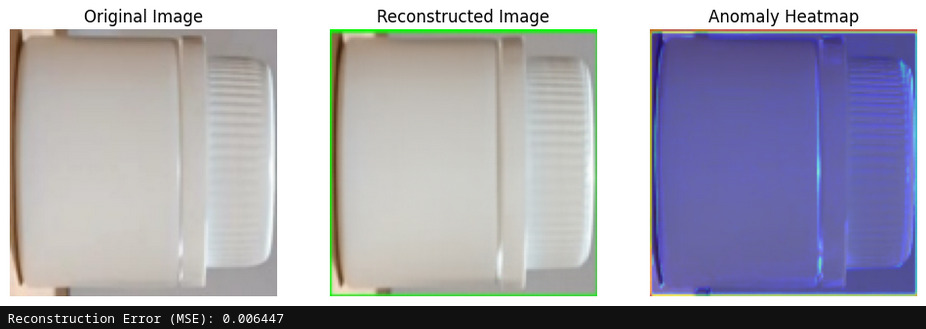
\includegraphics[width=\textwidth]{gambar/kontainer_bagus.jpeg}
    (a)
  \end{minipage}
  \vspace{1em}

  % Second image
  \begin{minipage}{\textwidth}
    \centering
    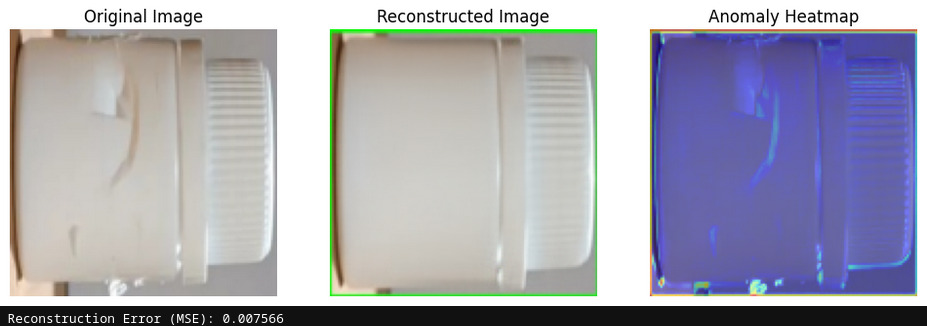
\includegraphics[width=\textwidth]{gambar/kontainer_cacat.jpeg}
    (b)
  \end{minipage}
  \caption{Hasil prediksi kecacatan: (a) Kontainer normal, (b)
  kontainer cacat}
  \label{fig:autoencoder-test}
  \vspace{-1em}
\end{figure}

Gambar di atas menunjukkan rekonstruksi \textit{error} model
\textit{autoencoder} pada kontainer normal dan cacat. Pada kontainer
normal, \textit{error} yang diperoleh adalah 0,006447 sedangkan pada
kontainer cacat sebesar 0,007566. Dari hasil tersebut terlihat
\textit{error} pada kontainer cacat lebih besar dibandingkan
\textit{error} pada kontainer normal. Hal ini menunjukkan bahwa model
sudah dapat membedakan kontainer normal dan cacat.

\vspace{1em}

\subsection{Penentuan Ambang Batas Kecacatan}
Penentuan ambang batas sangat penting agar sistem deteksi cacat dapat
membedakan secara akurat antara kontainer kimia yang cacat dan yang
normal. Tanpa ambang batas yang tepat, model berpotensi menghasilkan
banyak kesalahan prediksi, sehingga mengurangi keandalan sistem.
Dalam penelitian ini, metrik \textit{error} yang digunakan untuk
mengukur perbedaan antara citra asli dan hasil rekonstruksi adalah
\textit{Mean Squared Error} (MSE).

MSE merupakan metrik yang paling umum digunakan untuk mengukur
kualitas citra secara kuantitatif. MSE menghitung rata-rata selisih
kuadrat antara piksel citra asli (\textit{input}) dengan piksel citra hasil
rekonstruksi (\textit{output}). Semakin kecil nilai MSE, semakin mirip citra
hasil rekonstruksi dengan citra aslinya, yang berarti model berhasil
meminimalkan distorsi \citep{27}. MSE dirumuskan sebagai berikut:

\begin{equation}
  MSE = \frac{1}{n} \sum_{i=1}^{n} (x_i - \hat{x}_i)^2
\end{equation}

Pengujian dilakukan pada 20 gambar kontainer kimia, terdiri dari 10
gambar kontainer normal dan 10 gambar kontainer cacat. Dari pengujian
ini diperoleh distribusi nilai MSE masing-masing gambar untuk
dianalisis lebih lanjut. Hasil perhitungan MSE pada 20 gambar uji
tersebut dirangkum pada Tabel \ref{tab:error-samples}.

\begin{table}[H]
  \centering
  \caption{Nilai \textit{error} untuk setiap sampel}
  \label{tab:error-samples}
  \begin{tabular}{ccc}
    \toprule
    \textbf{No} & \textbf{Error} & \textbf{Kategori} \\
    \midrule
    1  & 0,006737 & Normal \\
    2  & 0,006828 & Normal \\
    3  & 0,007091 & Normal \\
    4  & 0,006997 & Normal \\
    5  & 0,006610 & Normal \\
    6  & 0,006795 & Normal \\
    7  & 0,006872 & Normal \\
    8  & 0,006725 & Normal \\
    9  & 0,006873 & Normal \\
    10 & 0,006817 & Normal \\
    11 & 0,007432 & Cacat \\
    12 & 0,007455 & Cacat \\
    13 & 0,008369 & Cacat \\
    14 & 0,007183 & Cacat \\
    15 & 0,007653 & Cacat \\
    16 & 0,008856 & Cacat \\
    17 & 0,007531 & Cacat \\
    18 & 0,007624 & Cacat \\
    19 & 0,007457 & Cacat \\
    20 & 0,008424 & Cacat \\
    \bottomrule
  \end{tabular}
\end{table}

Tabel \ref{tab:error-samples} menyajikan nilai \textit{error} atau
selisih rekonstruksi pada masing-masing sampel gambar, yang terdiri
dari 10 kontainer normal dan 10 kontainer cacat. Terlihat bahwa
sampel kategori normal memiliki nilai \textit{error} yang relatif
kecil dan cukup seragam, rata-rata sekitar 0,0067. Hal ini
menunjukkan bahwa model mampu merekonstruksi kontainer normal dengan
baik. Sebaliknya, sampel kategori cacat memperlihatkan nilai
\textit{error} yang cenderung lebih tinggi. Nilai \textit{error} yang
besar ini mengindikasikan adanya perbedaan signifikan pada area
cacat, yang gagal direkonstruksi secara sempurna oleh model, sehingga
mempermudah proses deteksi anomali.

\begin{equation}
  J = \textit{True Positive Rate} - \textit{False Positive Rate}
\end{equation}

Kurva \textit{Receiver Operating Characteristic} (ROC) digunakan
sebagai metode analisis untuk mengevaluasi performa model deteksi
cacat pada kontainer kimia dalam penelitian ini. Kurva ROC dibuat
dengan memplot nilai 1 - \textit{specificity} (\textit{false positive
rate}) pada sumbu-x dan \textit{recall} (\textit{true positive rate})
pada sumbu-y untuk setiap nilai ambang batas yang diuji.
\textit{Specificity} sendiri adalah ukuran seberapa baik model dalam
mengenali data negatif secara benar. Nilai ambang batas
terbaiki ditentukan dengan memaksimalkan statistik Youden J, yang
dirumuskan pada Persamaan 6
\citep{28}. Kurva ROC yang menggambarkan kinerja model secara
menyeluruh dapat dilihat pada Gambar \ref{fig:roc}.

\begin{figure}[H]
  \centering
  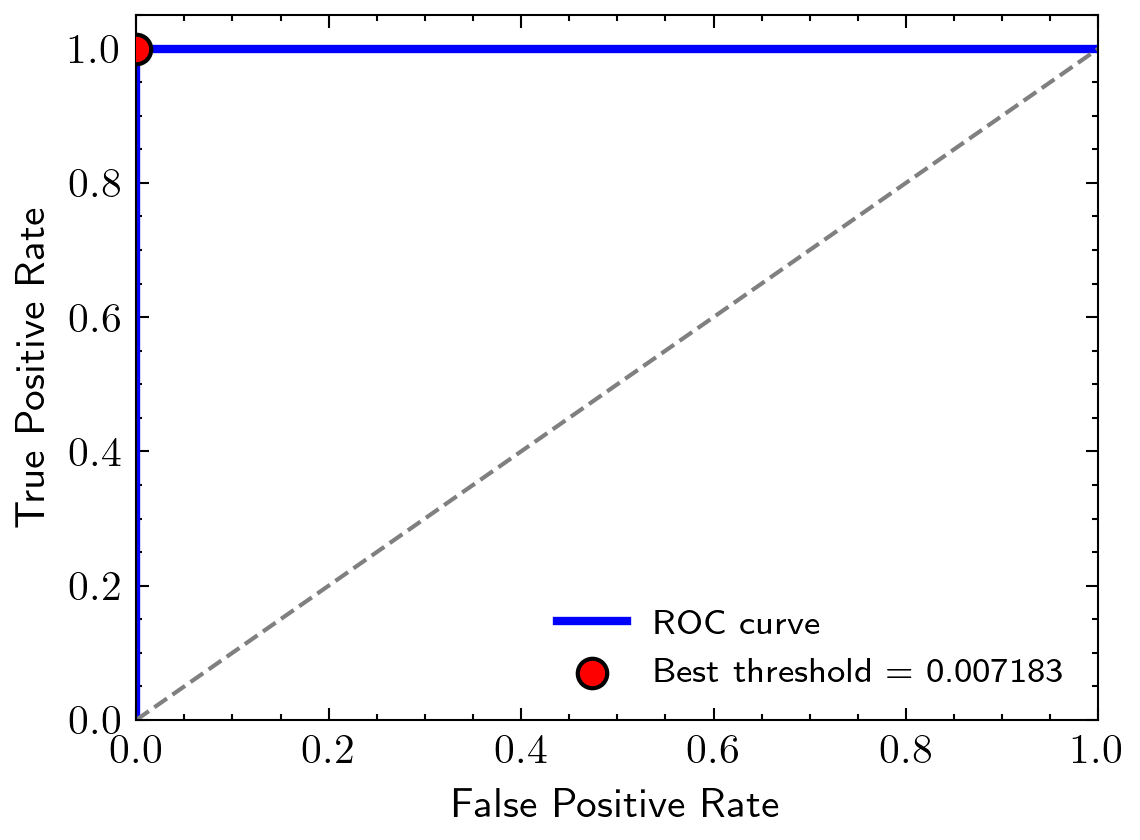
\includegraphics[width=\textwidth]{gambar/roc.png}
  \caption{Kurva ROC}
  \label{fig:roc}
\end{figure}
\vspace{-1em}

Kurva di atas menunjukkan performa model dalam membedakan kontainer
cacat dan tidak dengan sangat baik, ditunjukkan oleh garis biru
yang mendekati titik sudut kiri atas. Berdasarkan perhitungan,
ambang batas optimal yang diperoleh adalah sebesar 0,007183, ditandai
dengan lingkaran merah pada grafik. Nilai ini digunakan sebagai batas
deteksi akhir, sehingga model dapat memaksimalkan sensitivitas
sekaligus meminimalkan kesalahan positif dalam identifikasi cacat.

\vspace{1em}

\section{Hasil Pengujian Sistem Lengan Robot}

Setelah model deteksi terlatih dan nilai ambang batas optimal
ditentukan, tahap selanjutnya adalah integrasi sistem dengan lengan
robot yang dikontrol oleh mikrokontroler Arduino. Berdasarkan hasil
klasifikasi dari model, lengan robot secara otomatis memindahkan
kontainer kimia. Objek akan diarahkan ke sebelah kiri jika sistem
mengidentifikasinya sebagai cacat, dan ke sebelah kanan jika
dinyatakan normal. Gambar \ref{fig:robot-only} mengilustrasikan aksi
lengan robot ketika sedang menyortir objek yang teridentifikasi cacat.

\begin{figure}[H]
  \centering
  % First image
  \begin{minipage}{\textwidth}
    \centering
    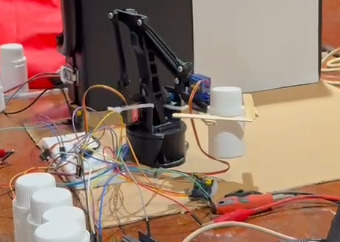
\includegraphics[width=0.88\textwidth]{gambar/robot_normal.jpeg}\\
    (a)
  \end{minipage}
  \vspace{1em}

  % Second image
  \begin{minipage}{\textwidth}
    \centering
    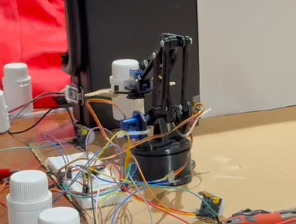
\includegraphics[width=0.88\textwidth]{gambar/robot_cacat.jpeg}\\
    (b)
  \end{minipage}
  \caption{Lengan robot menyortir kontainer: (a) normal, (b) cacat}
  \label{fig:robot-only}
  \vspace{-1em}
\end{figure}

Setelah lengan robot melepaskan kontainer di area penyortiran yang
telah ditentukan, sebuah sensor PIR yang terpasang di lokasi tersebut
akan mendeteksi keberadaan objek. Deteksi dari sensor PIR ini berfungsi
sebagai sinyal konfirmasi bahwa satu siklus penyortiran telah
selesai. Sinyal ini kemudian memicu pengiriman data hasil
klasifikasi, yang mencakup citra kontainer beserta label statusnya,
ke \textit{web server}. Untuk menampilkan informasi ini secara
\textit{real-time} kepada klien, sistem memanfaatkan protokol
\textit{WebSocket}. Tampilan website dan hasil prediksi dapat dilihat
pada Gambar
\ref{fig:web-test}.

\begin{figure}[H]
  \centering
  % First image
  \begin{minipage}{\textwidth}
    \centering
    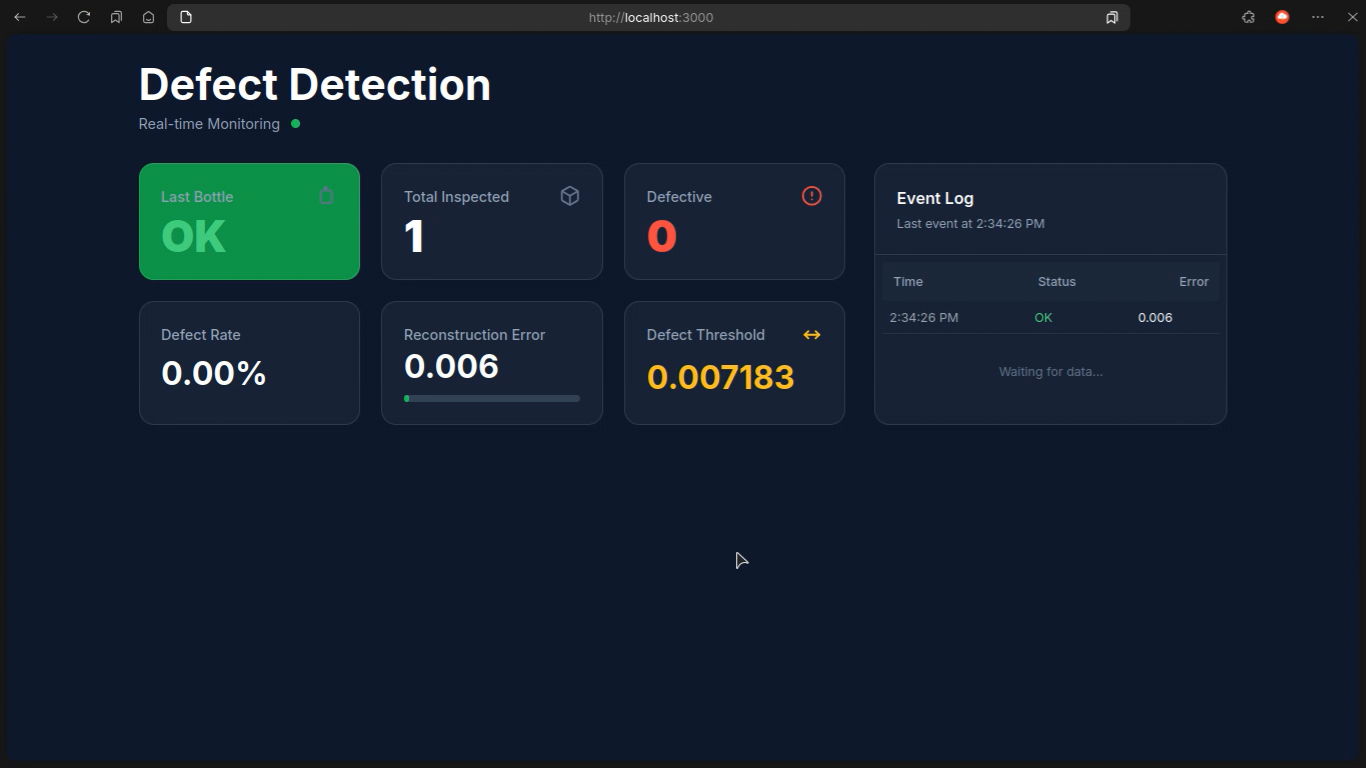
\includegraphics[width=\textwidth]{gambar/web_ss_normal.png}
    (a)
  \end{minipage}
  \vspace{1em}

  % Second image
  \begin{minipage}{\textwidth}
    \centering
    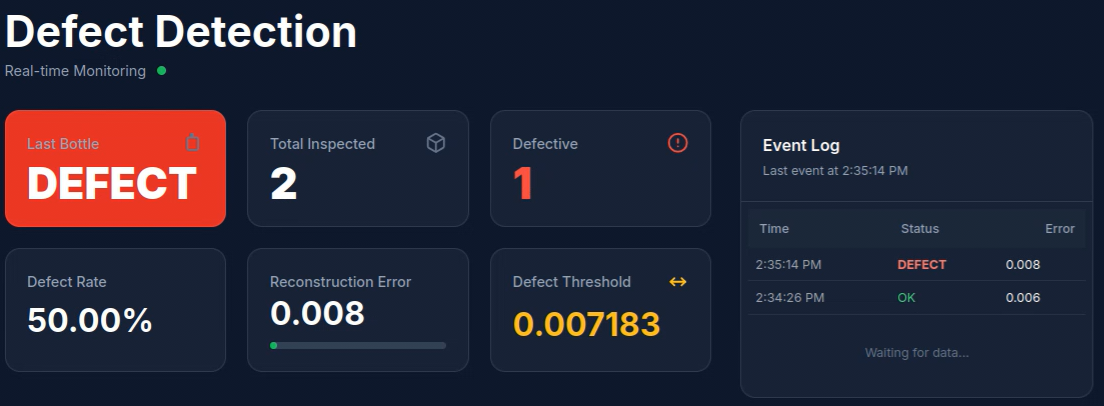
\includegraphics[width=\textwidth]{gambar/web_ss_cacat.png}
    (b)
  \end{minipage}
  \centering
  \caption{Tampilan hasil prediksi melalui \textit{website}: (a)
  kontainer normal, (b) kontainer cacat}
  \label{fig:web-test}
  \vspace{-1em}
\end{figure}

Untuk menguji keandalan dan konsistensi performa model, dilakukan
serangkaian pengujian sebanyak 25 kali pada objek kontainer. Setiap
pengujian menggunakan sampel dengan kondisi yang bervariasi antara
normal dan cacat untuk mengevaluasi kemampuan generalisasi model.
Hasil kuantitatif dari setiap pengujian ini dirangkum secara rinci
pada Tabel \ref{tab:error-samples-web}.

\begin{table}[H]
  \centering
  \caption{Nilai \textit{error} untuk setiap sampel uji}
  \label{tab:error-samples-web}
  \begin{tabular}{cccc}
    \toprule
    \textbf{No} & \textbf{Error} & \textbf{Kategori
      (Ambang Batas <
    0,007183)} & \textbf{Label Asli} \\
    \midrule
    1  & 0,006798 & Normal & Normal \\
    2  & 0,008298 & Cacat & Cacat \\
    3  & 0,006854 & Normal & Normal \\
    4  & 0,007066 & Normal & Normal \\
    5  & 0,006923 & Normal & Normal \\
    6  & 0,007607 & Cacat & Cacat \\
    7  & 0,007261 & Cacat & Cacat \\
    8  & 0,007393 & Cacat & Cacat \\
    9  & 0,006842 & Normal & Normal \\
    10 & 0,008099 & Cacat & Cacat \\
    11 & 0,006945 & Normal & Normal \\
    12 & 0,007381 & Cacat & Cacat \\
    13 & 0,006722 & Normal & Normal \\
    14 & 0,006865 & Normal & Normal \\
    15 & 0,007397 & Cacat & Cacat \\
    16 & 0,007099 & Normal & Normal \\
    17 & 0,006790 & Normal & Normal \\
    18 & 0,006760 & Normal & Normal \\
    19 & 0,007383 & Cacat & Cacat \\
    20 & 0,007693 & Cacat & Cacat \\
    21 & 0,008071 & Cacat & Cacat \\
    22 & 0,007977 & Cacat & Cacat \\
    23 & 0,006885 & Normal & Normal \\
    24 & 0,008007 & Cacat & Cacat \\
    25 & 0,006847 & Normal & Normal \\
    \midrule
    \multicolumn{3}{r}{\textbf{Tingkat Akurasi}} & \textbf{100\%} \\
    \bottomrule
  \end{tabular}
\end{table}

Tabel \ref{tab:error-samples-web} menyajikan hasil pengujian
performa model deteksi kecacatan pada 25 sampel kontainer yang
berbeda untuk memvalidasi efektivitasnya. Keputusan klasifikasi untuk
setiap sampel didasarkan pada perbandingan nilai \textit{error} rekonstruksi
terhadap ambang batas yang telah ditentukan sebesar
0,007183. Sesuai dengan mekanisme ini, objek dengan nilai \textit{error} di
bawah ambang batas dikategorikan sebagai "Normal", sementara objek
dengan nilai \textit{error} yang melebihinya dikategorikan sebagai "Cacat".
Hasil pada tabel secara jelas menunjukkan bahwa untuk keseluruhan 25
data uji, kolom "Kategori" (label prediksi dari model) sepenuhnya
konsisten dengan kolom "Label Asli" (\textit{ground truth}). Sebagai
contoh, pada data no. 2, nilai \textit{error} yang tinggi (0,008298)
berhasil diidentifikasi dengan benar sebagai "Cacat", sementara pada
data no. 1, nilai \textit{error} yang rendah (0,006798) juga tepat
diklasifikasikan sebagai "Normal". Kesesuaian antara
prediksi dan kondisi sebenarnya pada seluruh rangkaian pengujian ini
membuktikan bahwa model, dengan ambang batas yang dipilih, mampu
mencapai tingkat akurasi 100\% dalam membedakan antara kontainer
normal dan cacat. Gambar \ref{fig:web-25} menampilkan hasil \textit{website}
setelah melakukan prediksi terhadap 25 sampel yang juga menunjukkan
hasil yang sama dengan Tabel \ref{tab:error-samples-web}.

\begin{figure}[H]
  \centering
  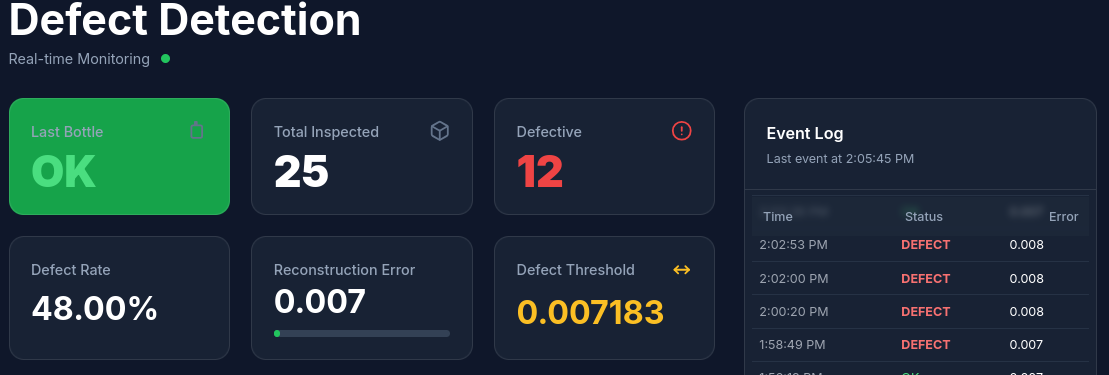
\includegraphics[width=\textwidth]{gambar/ss_web_25.png}
  \caption{Hasil prediksi kecacatan pada 25 sampel}
  \label{fig:web-25}
\end{figure}
\vspace{-1em}
